\documentclass[a4paper,10pt,titlepage]{article}
\usepackage[brazilian]{babel}
\usepackage[utf8]{inputenc}
\usepackage[ruled,linesnumbered]{algorithm2e}
\usepackage[table,xcdraw]{xcolor}
\usepackage{graphics} 
\usepackage{epsfig} 
\usepackage{amsmath} 
\usepackage{amssymb}  
\usepackage{nicefrac}
\usepackage{subfig}
\usepackage{setspace}
\usepackage{microtype}
\usepackage{color}
\usepackage{listings,xcolor}
\usepackage{ragged2e}
\usepackage{times}
\usepackage{multicol}
\usepackage{tabularx}
\usepackage{geometry}
\geometry{
 a4paper,
 total={170mm,257mm},
 left=20mm,
 top=20mm,
 }
 
\begin{document} 

\newcommand{\HRule}{\rule{\linewidth}{0.5mm}}
\HRule
\begin{large}
    \begin{justify}
        \begin{onehalfspace}
    \begin{center}
        \textbf{REDAÇÃO EMPRESARIAL: RELATÓRIO DE ROTINA ADMINISTRATIVA}\\[0.5cm]
    \end{center}
            \noindent O presente relatório tem por objetivo documentar as rotinas empresariais executadas por (Nome), jovem aprendiz do setor administrativo da empresa do ramo imobiliário (EMPRESA), localizada na cidade de (Cidade), que atua sob supervisão do tutor (Nome). As atividades foram empreendidas no período de 30 (trinta) de Agosto a 02 (dois) de Setembro do ano de 2021 (dois mil e vinte um).\\
            
            \noindent Havendo uma demanda por um relatório de período de \textbf{vacância}\footnote[1]{Condição ou estado do que não se encontra ocupado ou preenchido} dos imóveis, a principal meta dessa semana vigente de trabalho voltou-se para a finalização de uma planilha otimizada dos contratos de locação dos patrimônios imobiliários da empresa. Em razão de não haver um repositório digital ou banco de dados com essas informações, excluiu-se a possbilidade de \textbf{mineração de dados}\footnote[2]{Processo de encontrar anomalias, padrões e correlações em grandes conjuntos de dados para prever resultados.}. Outra adversidade identificada era a formatação do relatório, considerando o volume de dados a serem armazenados e interpretados graficamente. Portanto, visando superar esses obstáculos, optou-se por dividir a base de dados do relatório em três partes: uma base de dados na qual \textbf{cada linha armazenaria a situação ocupacional mensal de cada imóvel}; seguida por um relatório sintetizado responsável por \textbf{parametrizar os dados}; e por fim uma \textit{dashboard}\footnote[3]{Painel de controle que expõe informações de forma simplificada e ajuda na tomada de decisões rápidas em um negócio.} para \textbf{apresentação}. Com a arquitura estruturada, a sondagem manual dos dados continuou a ser realizada, sendo feita a apuração dos contratos através da leitura e digitalizando os mesmos pelo \textit{software} de planilhas Excel.
        \end{onehalfspace}
    \end{justify}
\end{large}
        
\begin{figure}[ht]\caption{Gráfico - Simulação do Relatório de Vacância}
    \centering
        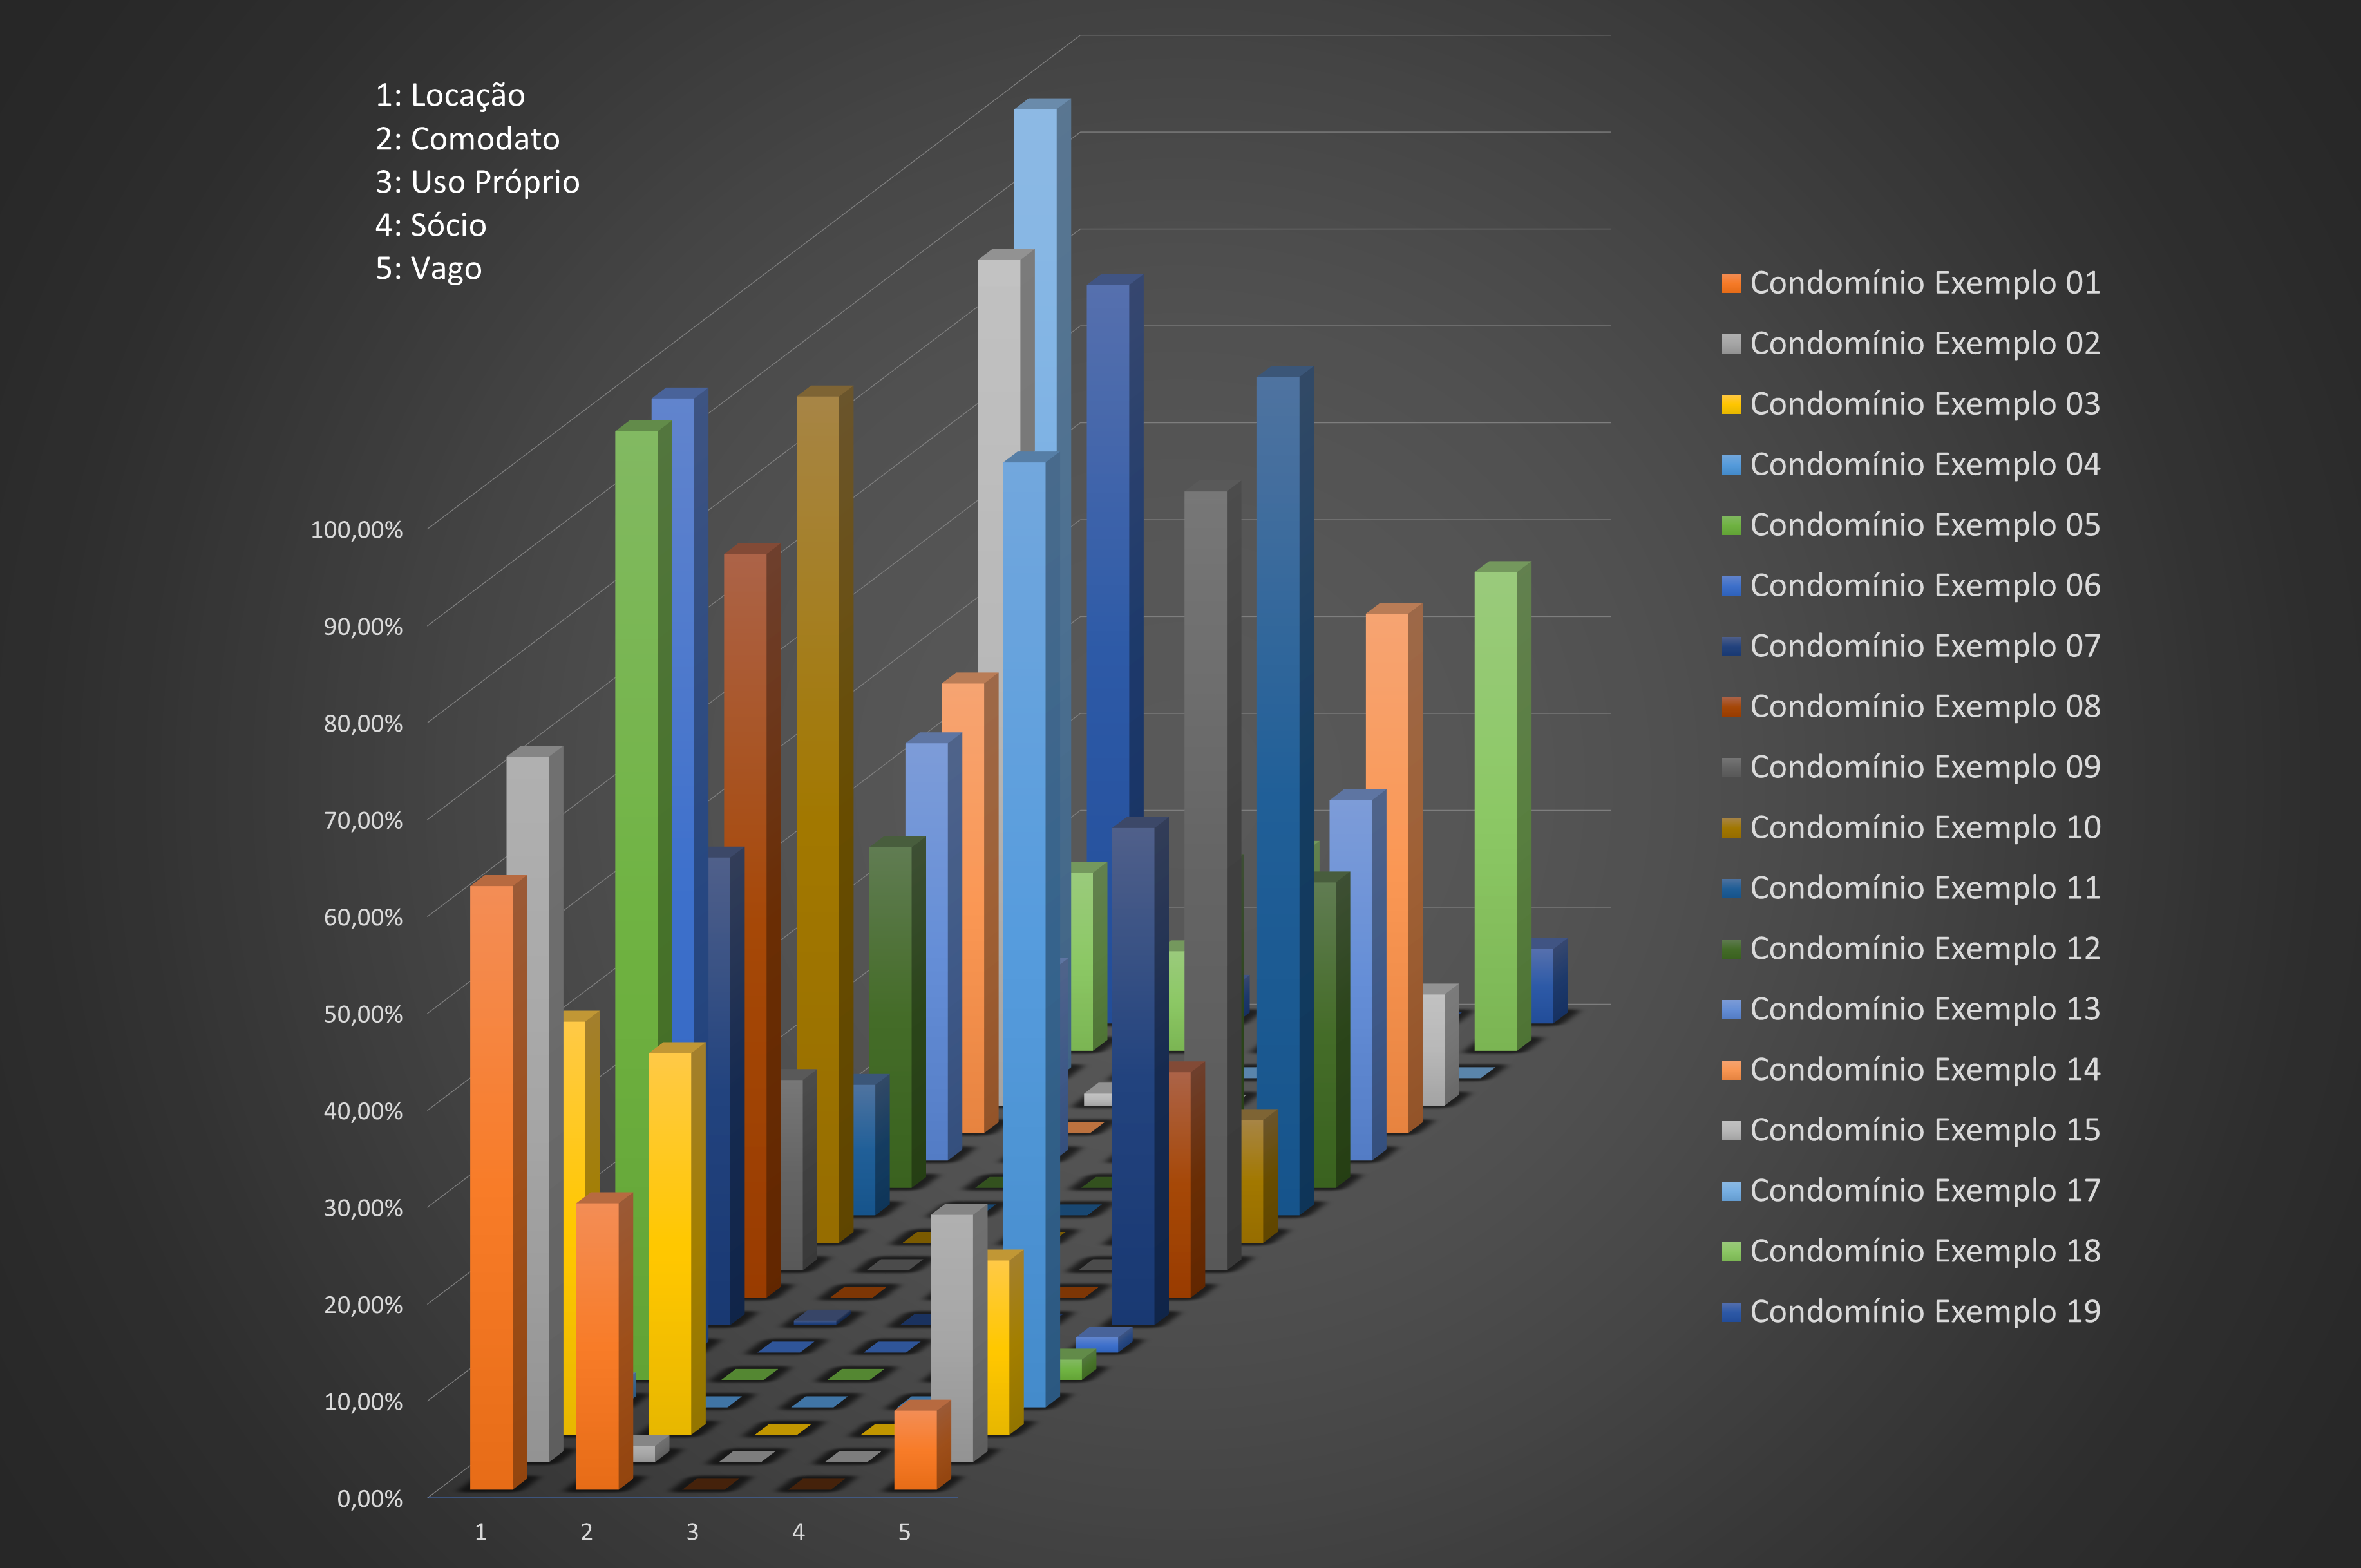
\includegraphics[scale = 0.3]{images/relatorio-vacancia.png}
        \label{figure:grafico-vacancia}
\end{figure}
    \begin{small}
        Fonte: adaptado de Vitória Peçanha de Araújo (2021).\\
    \end{small}
    
\begin{large}
    \begin{justify}
        \begin{onehalfspace}
            \noindent A entrega do relatório ocorreu ao segundo dia do mês de Setembro, \textbf{dentro do prazo estipulado pela gestão}. Por meio da execução desse projeto foi possível aprofundar os conhecimentos acerca da cronologia do patrimônio da empresa, bem como se familiarizar com novos conceitos e trâmites de locação de imóveis.\vfill
        \end{onehalfspace}
    \end{justify}
\end{large}

\end{document}
